\documentclass[12pt]{article}
\usepackage[T1]{fontenc}
\usepackage[utf8]{inputenc}
\usepackage{helvet}
\renewcommand{\familydefault}{\sfdefault}
\usepackage[a4paper,margin=24mm,headheight=16pt]{geometry}
\usepackage{microtype}
\usepackage{amsmath,amssymb,amsthm,mathtools}
\usepackage{graphicx,booktabs,tabularx,array,longtable}
\usepackage{caption,placeins,float}
\usepackage[numbers,sort&compress]{natbib}
\setlength{\bibsep}{3pt}
\usepackage{fancyhdr,xurl}
\usepackage[hidelinks,breaklinks=true]{hyperref}
\hypersetup{pdftitle={From correction capacity to correction control: operator-aware evaluation of image restoration},pdfauthor={Ruizi Wang},pdfsubject={Liaoning Vocational College of Light Industry; email: 454762251@qq.com; ORCID: 0000-0002-6646-9907}}
\captionsetup{font=normalsize,labelfont=bf,skip=8pt,labelsep=space}
\captionsetup[figure]{name=Fig.}
\captionsetup[table]{position=above}
\renewcommand{\footnotesize}{\normalsize}
\setlength{\parskip}{4pt}
\setlength{\parindent}{1.1em}
\setlength{\emergencystretch}{3em}
\setlength{\tabcolsep}{5pt}
\renewcommand{\arraystretch}{1.16}
\widowpenalty=10000\clubpenalty=10000\displaywidowpenalty=10000
\renewcommand{\topfraction}{0.94}\renewcommand{\bottomfraction}{0.85}
\renewcommand{\textfraction}{0.05}\renewcommand{\floatpagefraction}{0.75}
\setcounter{topnumber}{3}\setcounter{totalnumber}{5}
\setcounter{secnumdepth}{2}\setcounter{tocdepth}{2}
\pagestyle{fancy}\fancyhf{}
\fancyhead[L]{Correction capacity and correction control}
\fancyfoot[C]{\thepage}
\newcommand{\MSE}{\operatorname{MSE}}
\newcommand{\PSNR}{\operatorname{PSNR}}
\newcommand{\clip}{\operatorname{clip}}
\newcommand{\softmax}{\operatorname{softmax}}
\newcommand{\mean}{\operatorname{mean}}
\newcommand{\RMS}{\operatorname{RMS}}
\newcommand{\JOME}{JOME}
\newcommand{\PAST}{PAST}
\newcommand{\ARISE}{ARISE}
\newcommand{\tabnote}[1]{\par\vspace{5pt}\noindent #1}
\newtheorem{proposition}{Proposition}
\newtheorem{corollary}{Corollary}
\newcolumntype{L}[1]{>{\raggedright\arraybackslash}p{#1}}

\providecommand{\doi}[1]{\url{https://doi.org/#1}}

\title{\bfseries From correction capacity to correction control:\\ operator-aware evaluation of image restoration}
\author{Ruizi Wang\\
\normalsize Liaoning Vocational College of Light Industry\\
\normalsize \href{mailto:454762251@qq.com}{454762251@qq.com}\\
\normalsize ORCID: \href{https://orcid.org/0000-0002-6646-9907}{0000-0002-6646-9907}}
\date{}
\begin{document}
\maketitle
\begin{abstract}
Image restoration combines the generation of candidate edits, their aggregation, and intervention on an observed image. We introduce an operator-aware evaluation framework that makes these stages separately testable through matched inference operators, loss-specific calibrated controls, and input-relative geometry. The framework characterizes bounded-action reachability, clipping-order discrepancies, and sufficient statistics for replaying global output-mixture losses. A four-expert residual system provides controlled evidence on 800 reflection-removal image pairs, complemented by 2,100 released-output geometry records. Uniform residual aggregation reproduces 95.6\% of the official-validation mean refinement gain. Under matched clipping, adaptive weighting adds 0.0073 dB (95\% image-bootstrap interval $[-0.0005,0.0150]$), while base-relative losses exceeding 0.1 dB decrease from 25 images to 12. Loss-specific calibration changes the comparison: a mean-PSNR-calibrated fixed mixture narrows the adaptive-output increment to 0.0034 dB, whereas MSE calibration selects a single expert. Twenty-one cross-candidate scalar products per image support both calibration objectives without repeating network inference. Measured input-recovery bounds connect preservation of the observation to the base-centered action region. On eight official near-identity inputs, all eight JOME edits align positively with the reference displacement, yet their median reference-optimal strength is 0.109. These results connect useful correction capacity to the operator, loss objective, and action set governing restoration control, and provide a reusable evidence specification for evaluating those decisions.
\end{abstract}
\noindent\textbf{Keywords:} image restoration; reflection removal; residual experts; evaluation methodology; input preservation; reproducibility.
\section{Introduction}
\label{sec:introduction}
Image restoration changes the evidence available to subsequent interpretation. Every edit selects which structures, intensities, and textures survive in the output. Reflection removal makes this choice particularly consequential: suppressing a superposed scene can also alter a legitimate transmitted structure. Variation in reflection formation, glass properties, and imaging conditions places correction strength and content preservation at the center of the problem \citep{wan2023benchmark,wen2019linearity,zheng2021absorption}.

Modern restoration systems distribute this task across cooperating streams, refinement stages, expert mixtures, and diffusion priors \citep{wan2020corrn,li2020cascaded,park2026complementary,hu2026dereflection}. Candidate generators determine which edits are available, aggregation determines how those edits interact, and the complete pipeline determines the displacement from the observation. An increase in final accuracy can arise at any of these stages. Connecting performance to the operation that produced it is therefore essential to deciding which components to retain, which controls to expose, and which experimental evidence to preserve.

We introduce an \emph{operator-aware evaluation framework} that connects three properties of a restoration system. \emph{Correction capacity} concerns the useful predictions available from a trained candidate bank. \emph{Aggregation behavior} concerns the effect of the implemented combination rule under a declared loss. \emph{Input-relative control} concerns the consequences of changing the observation and the availability of an unchanged-input action. These properties become separately testable through matched inference operators, loss-specific fixed controls, and comparisons against both the base prediction and the input. A compact cross-candidate loss record makes an important family of these comparisons replayable after model execution.

A jointly optimized mixture of residual experts, JOME, provides the experimental realization. Four homogeneous branches generate bounded corrections around a frozen spectral--phase restoration backbone, and a spatial router combines their outputs. The system contains 24.76 million parameters, including a 3.03-million-parameter correction stage. The fixed backbone exposes candidate generation and aggregation in a common experimental setting, complementing lightweight unfolding and reflection-specific expert architectures \citep{huang2025dexnet,park2026complementary}.

A controlled inference pass on 800 image pairs makes the evaluation framework operational. Crossing adaptive versus uniform weights with clipping before versus after aggregation separates the weighting effect from implementation order. On official validation, uniform residual aggregation reproduces 95.6\% of the mean refinement gain. Adaptive weighting contributes a further 0.0073 dB, while the weighting-by-clipping interaction is approximately $1.24\times10^{-5}$ dB. Its clearest distributional effect is a reduction in base-relative losses exceeding 0.1 dB, from 25 images to 12. This pairing of a small mean increment with a larger change in the loss distribution gives aggregation a more informative characterization than an aggregate score alone.

Calibrated controls sharpen that characterization. The global four-expert mixture minimizing selection-partition mean image MSE reduces to one expert. A mixture calibrated for mean PSNR assigns weight to three experts and narrows the official adaptive-output advantage to 0.0034 dB. Extending calibration to include the base and input changes the available actions and produces further shifts in the comparison. These alternatives are evaluated directly from 21 cross-candidate scalar products per image. The experiment connects the choice of evidence to the ability to test a stronger baseline, and connects that baseline to the loss objective it represents.

Input-relative evaluation reveals a second design issue. Six official raw outputs improve the base while remaining worse than the input. A bounded correction stage explores a neighborhood around its base prediction; the original observation can lie outside that neighborhood. We derive the resulting input-recovery bound and measure its activity and magnitude, then connect the observed edits to their direction, strength, and reference-space margins. In the eight official inputs with PSNR at least 40 dB, every JOME edit aligns positively with the reference displacement, yet the median reference-optimal edit strength is only 0.109. This geometry identifies where action availability and action selection become consequential.

The paper contributes a unified measurement framework, a replayable evidence specification, and an empirical analysis that exercises both. The framework supplies exact gain accounting, matched weighting--clipping comparisons, and bounded-action reachability. The evidence specification includes a constructive scalar-score insufficiency result and sufficient statistics for evaluating global output mixtures under multiple losses. The empirical study combines 800 controlled raw-output records, calibration-selected alternatives, and 2,100 released-output geometry records to show how candidate value, aggregation, and input-relative outcomes interact. These contributions make a modular restoration result interpretable at the level of the predictions available, the operation deployed, and the observation changed.

\section{Correction, aggregation, and control in restoration}
\label{sec:related}
\subsection{Reflection formation, supervision, and compact restoration}
Reflection removal brings together image-formation assumptions, supervision design, and learned image priors. Ghosting cues reveal aspects of reflection structure \citep{shih2015ghosting}, while nonlinear formation and absorption models account for effects beyond a simple additive RGB mixture \citep{wen2019linearity,zheng2021absorption}. The journal benchmark of Wan et al. organizes evaluation across varied glass properties and capture conditions \citep{wan2023benchmark}. These perspectives establish the importance of specifying what a reference represents: a desired rendered appearance, a separately captured transmission image, or a quantity defined by a physical formation model.

Learned methods address the resulting ambiguity through complementary forms of supervision and information exchange. Perceptual-loss separation, misaligned-pair training, cascaded refinement, cooperative streams, and component synergy strengthen different parts of the restoration process \citep{zhang2018reflection,wei2019misaligned,li2020cascaded,wan2020corrn,hu2021trash,hu2023synergy}. Location-aware processing connects spatial variation in reflection evidence to the restoration operation \citep{dong2021location}. Related spatial adaptation appears in single-image raindrop removal: Fu et al. combine top-$k$ sparse attention with an uncertainty-guided training loss to address sparse, spatially varying degradation \citep{fu2024ustn}. Our fixed-backbone design makes the predictions of jointly trained residual branches available for direct comparison under alternative aggregation rules. The branches learn from a shared final-output objective, with branch identities serving as computational indices.

Compact architectures and stronger priors provide complementary routes to restoration quality. DExNet translates a structured separation model into a lightweight deep exclusion-unfolding network \citep{huang2025dexnet}. Dereflection Any Image combines diversified data acquisition with one-step diffusion and reflection-invariant training \citep{hu2026dereflection}; RefMover introduces language and region guidance into diffusion-based reflection removal \citep{wang2026refmover}. Transferable priors also extend across restoration tasks: UniFMIR combines pretraining with task-specific fine-tuning for fluorescence-microscopy image restoration \citep{ma2024unifmir}. Across these approaches, performance improvements arise through architecture, training data, and conditioning. Our evaluation framework adds a measurement perspective: it asks how much of a realized improvement is available in the candidates, how aggregation changes their loss profile, and how the complete result compares with the observation. The quantitative external comparisons in this paper use the released outputs identified in Section~\ref{sec:protocol}.

Additional measurements also change the information available to the restoration system. RAW-domain methods retain a less processed signal, and flash-only or polarization cues provide supplementary evidence about the scene \citep{kee2025raw,lei2023flash,yao2025polarfree}. Their connection to our study concerns identifiability and reference construction; the implemented evaluation uses a single rendered RGB input. OpenRR's edited references provide a further supervision setting \citep{cai2025openrr}. Keeping acquisition and target construction explicit makes comparisons across these settings scientifically interpretable.

\subsection{Residual experts and aggregation evidence}
Residual learning has established roles in recognition and image restoration \citep{he2016resnet,zhang2017dncnn}. Mixtures of experts organize adaptive combinations of predictors, from early ensemble formulations to large conditional-computation systems \citep{jacobs1991adaptive,shazeer2017outrageously}. Their evaluation involves several separable properties: differentiation between candidates, the quality of the aggregation rule, and the execution pattern that determines computational cost.

Restoration-specific expert designs make these distinctions concrete. MoCE-IR uses complexity-differentiated experts \citep{zamfir2025moce}, while Park and Sim use complementary experts with spatial assignment for reflection separation \citep{park2026complementary}. JOME instead uses homogeneous, jointly trained residual branches around a fixed estimate. All branches execute before aggregation. This design supports an inference comparison within one co-adapted candidate bank, while semantic differentiation and execution efficiency remain separately measurable properties.

Ensemble theory and calibrated combinations provide analytical starting points. Stacked regression learns nonnegative predictor combinations from held-out predictions, making the fitting objective and calibration design explicit \citep{breiman1996stacked}. The ambiguity identity connects the squared error of an average prediction to average individual error and prediction diversity \citep{krogh1994ensembles}. An evaluation archive must additionally preserve the information needed for the mixtures researchers wish to compare. Candidate-wise scores contain self-errors; mixture losses also depend on cross-candidate error products. We develop this connection into a compact logging specification and a constructive identifiability result. The specification gives an exact family of replayable comparisons and relates it to nonlinear clipping and spatial weighting. The controlled study then uses that record to compare MSE-calibrated and PSNR-calibrated fixed mixtures with adaptive aggregation on the same predictions.

\subsection{Controllability, preservation, and reliable measurement}
Controllable restoration exposes decisions about the type and strength of an edit. CURE learns selective degradation removal, adjustable restoration strength, and an identity mode \citep{kim2026cure}. Such controls create an action space whose utility also depends on how actions are selected. Our framework treats action availability and input-relative outcome as distinct evaluation objects, linking both to the original observation and the chosen reference.

Selective prediction supplies a related perspective through acceptance and abstention \citep{elyaniv2010selective,geifman2019selectivenet}. In restoration, returning the input makes abstention a concrete image-valued action with a measurable loss. This invites risk--coverage analysis with an explicit input baseline. Predictive uncertainty and calibration provide tools for assessing decision quality \citep{lakshminarayanan2017ensembles,guo2017calibration}; distribution-free image-to-image methods further show how calibrated prediction sets can be constructed \citep{angelopoulos2022imaging}. These approaches motivate evaluating an action-selection rule using its deployment-available information and calibration protocol. The JOME experiments concern the observed consequences of aggregation and the reachability of candidate actions.

Image-quality metrics capture different aspects of an output. PSNR and structural similarity (SSIM) compare reference-based fidelity; LPIPS and DISTS introduce learned feature or structure--texture comparisons; NIQE supplies a reference-free measure \citep{wang2004ssim,zhang2018lpips,ding2020dists,mittal2013niqe}. Spatial importance introduces a further choice: Ardizzone and Bruno compare saliency-weighted fidelity measures with their unweighted counterparts and examine their relationship to subjective quality judgments \citep{ardizzone2012saliency}. Perception--distortion and perception--robustness results describe related tensions in restoration \citep{blau2018perception,ohayon2024robustness}. Our analysis makes metric choice part of the evaluation by reporting logarithmic and arithmetic error aggregation alongside positive gains, losses, and input-relative strata.

Model-selection bias and underspecification further motivate transparent evaluation provenance \citep{cawley2010selection,damour2022underspecification}. We pair every result with the operator, baseline, representation, and comparison population that define it. Table~\ref{tab:questions} brings these elements together. This operational specification connects established restoration and evaluation literature to a reproducible assessment of what a particular correction system contributes.

\section{An operator-aware evaluation framework}
\label{sec:framework}
\subsection{Two baselines and four matched aggregation operators}
Let $I\in[0,1]^{H\times W\times3}$ be the observed input, $T$ the reference, and $B=f_\theta(I)$ a base restoration in the same image box. Let $P$ denote coordinatewise clipping to $[0,1]$. Norms and inner products below average over evaluated RGB samples after the declared border crop, so $\|X-T\|^2$ is an image MSE. For positive MSE,
\begin{equation}
\PSNR(X,T)=-10\log_{10}\|X-T\|^2.
\end{equation}

For residual candidates $r_k$, $k=0,\ldots,K-1$, define $z_k=P(B+r_k)$ and spatial convex weights $w_k$. Crossing weights and clipping order gives
\begin{align}
U_o &= K^{-1}\sum_k z_k, &
Y_o &= \sum_k w_k z_k, \label{eq:uniform-output}\\
U_r &= P\!\left(B+K^{-1}\sum_k r_k\right), \label{eq:uniform-residual}\\
Y_r &= P\!\left(B+\sum_k w_k r_k\right). \label{eq:routed}
\end{align}
Subscripts $o$ and $r$ identify output-space and residual-space aggregation. $Y_r-U_r$ changes weights at a fixed residual-then-clip operator; $Y_o-U_o$ changes weights after clipping the same candidates. The weights in $Y_o$ are the frozen router weights used in $Y_r$. This comparison evaluates the realized inference operation conditional on the trained candidate bank.

For a score $s$, the factorial interaction is
\begin{equation}
\mathcal I_s=[s(Y_r)-s(U_r)]-[s(Y_o)-s(U_o)]. \label{eq:interaction}
\end{equation}
Evaluating all four outputs identifies both weighting effects and the influence of clipping order on their difference. It also prevents a clipping change from being absorbed into a claimed weighting effect.

Write $Y=Y_r$ for the deployed prediction. Its base-relative and input-relative gains satisfy
\begin{align}
\Delta_B &= \PSNR(Y,T)-\PSNR(B,T),\\
\Delta_I &= \PSNR(Y,T)-\PSNR(I,T),\\
\Delta_I &= \Delta_B+\PSNR(B,T)-\PSNR(I,T). \label{eq:two-baselines}
\end{align}
The identity connects stagewise progress to the consequence of the complete edit. A refiner can repair part of a base error while the original input still has lower reference loss. The baseline representing an unchanged observation is therefore $I$; a zero residual represents an unchanged base $B$.

Using the matched residual-space uniform control, refinement gain has the exact accounting
\begin{align}
\Delta_{\rm bank} &= \PSNR(U_r,T)-\PSNR(B,T),\\
\Delta_{\rm weight} &= \PSNR(Y_r,T)-\PSNR(U_r,T),\\
\Delta_B &= \Delta_{\rm bank}+\Delta_{\rm weight}. \label{eq:accounting}
\end{align}
These are differences between inference outputs of a jointly trained system. Alternative training mechanisms can change the candidates themselves and are addressed by independently trained controls.

\begin{table}[t]
\caption{Evaluation questions and the evidence that makes them testable}
\label{tab:questions}
\begin{tabularx}{\linewidth}{@{}L{.22\linewidth}XX@{}}
\toprule
Question & Comparison & Required evidence\\
\midrule
Candidate value & Base, individual candidates, uniform and calibrated fixed mixtures & Candidate definitions and paired losses\\
Adaptive weighting & Same candidates, clipping order, representation, and loss objective & Four matched outputs; fixed-mixture controls\\
Input-relative outcome & Prediction versus input and base; conditional gain and loss profiles & Input, base, and output losses\\
Action availability & Input distance from the bounded correction region & Base--input displacement and amplitude envelope\\
Mixture replay & Calibration-selected global output weights, frozen on evaluation images & Per-image cross-candidate error Gram matrix\\
\bottomrule
\end{tabularx}
\end{table}

\subsection{Input reachability under bounded correction}
Suppose $|r_{k,j}|\leq\epsilon$ for every expert and evaluated RGB coordinate $j$, and weights are pointwise convex. Projection cannot increase a displacement from $B$ because $B$ already lies in the image box.
\begin{proposition}[Reachability of bounded base-centered correction]
\label{prop:reachability}
Every output of Eq.~\eqref{eq:routed} satisfies $|Y_j-B_j|\leq\epsilon$. For any desired image $X$,
\begin{equation}
\MSE(Y,X)\ \geq\ \frac{1}{m}\sum_{j=1}^{m}
\left(|B_j-X_j|-\epsilon\right)_+^2, \label{eq:reachable-bound}
\end{equation}
where $m$ is the number of evaluated RGB samples and $(a)_+=\max(a,0)$.
\end{proposition}
\begin{proof}
Convexity gives $|\sum_k w_{k,j}r_{k,j}|\leq\epsilon$. Projection is nonexpansive and leaves $B_j$ fixed, hence $|Y_j-B_j|\leq\epsilon$. The reverse triangle inequality gives $|Y_j-X_j|\geq(|B_j-X_j|-\epsilon)_+$. Squaring and averaging proves the bound.
\end{proof}
Taking $X=I$ gives a necessary condition for exact input recovery. A positive bound excludes $I$ from the nominal correction neighborhood. A zero bound places $I$ within the coordinate envelope; the actual candidate bank may span a smaller set. Thus bound activity, bound magnitude, and output preference under $T$ describe different properties. In particular, a useful restoration can have a large input-recovery bound when the desired edit itself is large.

The bound also identifies a direct action-space extension: including $I$ as a candidate makes the unchanged observation available regardless of its distance from $B$. The empirical analysis reports the nominal $\epsilon=0.1$ bound together with a numerical-envelope audit, preserving the distinction between exact arithmetic assumptions and recorded floating-point outputs.

\subsection{The scale of clipping-order discrepancies}
Let $x_k=B+r_k$. A coordinatewise bound is
\begin{equation}
|U_o-U_r|\ \leq\ K^{-1}\sum_k|P(x_k)-x_k|. \label{eq:clipping-coordinate}
\end{equation}
Indeed, $U_o$ lies in the image box, so $P(U_o)=U_o$; coordinatewise nonexpansiveness bounds its distance from $P(K^{-1}\sum_kx_k)$ by the average clipping displacement. Taking the root-mean-square norm gives
\begin{equation}
\|U_o-U_r\|\leq\left\|K^{-1}\sum_k|P(x_k)-x_k|\right\|
\leq K^{-1}\sum_k\|P(x_k)-x_k\|. \label{eq:clipping-bound}
\end{equation}
The first bound is evaluated in the controlled run. The mean absolute clipping displacement separately bounds mean absolute operator discrepancy; matching the norm is essential to the numerical check. For scalar $B=0.98$ and residuals $+0.10,-0.10$, $U_o=0.94$ while $U_r=0.98$. The magnitude of this effect in a trained system is measured by the matched outputs and Eq.~\eqref{eq:interaction}.

\subsection{Replayable mixture evaluation from cross-candidate evidence}
For clipped outputs, the ambiguity identity connects averaging to candidate diversity \citep{krogh1994ensembles}:
\begin{equation}
K^{-1}\sum_k\|z_k-T\|^2-\|U_o-T\|^2
=K^{-1}\sum_k\|z_k-U_o\|^2. \label{eq:ambiguity}
\end{equation}
Evaluating alternative global mixtures additionally requires their cross-candidate error structure. Define
\begin{equation}
G_{k\ell}=\langle z_k-T,z_\ell-T\rangle.
\end{equation}
For a simplex weight vector $\alpha$ constant across pixels,
\begin{equation}
\MSE\!\left(\sum_k\alpha_kz_k,T\right)=\alpha^\top G\alpha. \label{eq:gram}
\end{equation}
Candidate-wise MSEs supply the diagonal of $G$ and a uniform score supplies one additional quadratic constraint. Their cross-products carry further information.

\begin{proposition}[Scalar-score insufficiency]
\label{prop:gram}
Even for four candidates, their individual MSEs and the MSE of their uniform average do not determine the minimum MSE attainable by a global convex mixture.
\end{proposition}
\begin{proof}
Let $G_0=I_4$ and $G_t=I_4+tH$, where
\begin{equation}
H=\begin{pmatrix}0&1&-1&0\\1&0&0&0\\-1&0&0&0\\0&0&0&0\end{pmatrix},
\qquad 0<t<1/\sqrt{2}.
\end{equation}
The eigenvalues of $H$ are $\sqrt{2},-\sqrt{2},0,0$, so both matrices are positive definite. Their diagonals agree and, for $u=(1/4,1/4,1/4,1/4)$, $u^\top G_0u=u^\top G_tu=1/4$. The minimum simplex loss for $G_0$ is $1/4$. The feasible vector $\alpha=(1/4,1/4-t/4,1/4+t/4,1/4)$ gives $\alpha^\top G_t\alpha=1/4-t^2/8<1/4$. Positive semidefinite matrices are Gram matrices of error vectors; common rescaling around a midrange target embeds the construction in bounded image values while preserving the inequality. The same scalar scores are therefore compatible with different optimal mixture losses.
\end{proof}

For four experts, the base, and the input, a symmetric $6\times6$ matrix requires 21 scalar products per image. Storing these products with candidate names, crop, value range, and representation makes losses of global convex mixtures of those six output images replayable. Spatial weights and residual mixing followed by clipping require matched outputs or richer image-level records. This operator-specific specification determines which comparisons remain possible after inference.

\subsection{Loss-specific calibration and error distributions}
Fixed combinations have a long history in stacked regression \citep{breiman1996stacked}. Given calibration images $\mathcal C$, their objective can be made explicit:
\begin{align}
\widehat\alpha_{\rm M}
&=\arg\min_{\alpha\in\Delta_K}\frac{1}{|\mathcal C|}\sum_{i\in\mathcal C}\alpha^\top G_i\alpha,\label{eq:calibration-mse}\\
J_{\rm P}(\alpha)
&=\frac{1}{|\mathcal C|}\sum_{i\in\mathcal C}\log(\alpha^\top G_i\alpha),\label{eq:calibration-psnr}
\end{align}
where $\Delta_K$ is the probability simplex. Minimizing $J_{\rm P}$ maximizes mean PSNR. The MSE problem is a convex quadratic; the log-quadratic problem is solved numerically with multiple starts. Both use the same per-image Gram records, and the selected coefficients are frozen before evaluation on other partitions. We denote the fitted predictions by $F_K^{\rm M}$ and $F_K^{\rm P}$.

The distinction between these losses follows directly from PSNR aggregation. For per-image MSEs $m_{i,Y}$ and $m_{i,B}$,
\begin{equation}
\overline{\Delta_B}=10\log_{10}\!\left[
\left(\prod_{i=1}^{n}\frac{m_{i,B}}{m_{i,Y}}\right)^{1/n}\right]. \label{eq:geometric}
\end{equation}
Mean PSNR measures a geometric mean of error ratios. Arithmetic mean image MSE gives equal image weight to absolute squared error; pooled pixel MSE would additionally weight images by evaluated size. A fixed-mixture baseline therefore needs a declared loss objective as well as a declared action set.

For an image-wise gain $g_i$ against a stated baseline, we also report
\begin{align}
G^+&=n^{-1}\sum_i\max(g_i,0),&G^-&=n^{-1}\sum_i\max(-g_i,0),\\
\bar g&=G^+-G^-,&H(\tau)&=n^{-1}\sum_i\mathbf1\{g_i<-\tau\}.\label{eq:loss-profile}
\end{align}
The positive and negative parts identify whether a mean gain reflects greater upside, reduced losses, or both. Numerical thresholds such as 0.1 dB trace that distribution; perceptual or application-specific tolerances require their own validation.

\section{Residual-expert restoration around a fixed backbone}
\label{sec:method}
\subsection{Spectral--phase backbone and structured features}
The PAST backbone contains 21.737337 million parameters. It is a four-scale encoder--decoder with widths 48/96/192/384, encoder block counts 1/1/4, two bottleneck blocks, and decoder counts 4/1/1. Its local processing uses nonlinear-activation-free (NAF) blocks \citep{chen2022nafnet}. Frequency-domain and phase-sensitive operations supply structured features, drawing on established frequency processing and the structural importance of phase \citep{kong2023fftformer,oppenheim1981phase}. The complete base is shared across the correction configurations, providing a common source of structured features.

At quarter and eighth resolution, local Fourier modules use overlapping $16\times16$ windows, stride eight, Hann weighting, and eight channel groups. For a feature-window spectrum $\widehat F$, the learned allocation has the form
\begin{equation}
\widehat F_T=m_T\odot\widehat F,\quad
\widehat F_N=m_N\odot\widehat F,\quad
m_T=a+\delta,\quad m_N=1-m_T.
\end{equation}
Here $a$ is a learned allocation and the real and imaginary parts of the complex adjustment $\delta$ are bounded by 0.1. Local windows allow the allocation to vary spatially. Complementarity constrains the algebraic sum while allowing multiple latent allocations: $(F_T+u,F_N-u)$ preserves the same sum for any admissible $u$. We therefore interpret the streams as learned feature allocations.

The coarse phase pathway uses eight learned projections and normalized cross-spectral statistics. For projected features $u,v$, a generic normalized cross-spectrum is
\begin{equation}
\widehat C_{uv}=
\frac{\widehat u\,\overline{\widehat v}}
{|\widehat u\,\overline{\widehat v}|+\varepsilon}.
\end{equation}
Inverse transforms and local/global circular summaries contribute phase context, combined with coarse channel attention before decoder fusion. The resulting maps encode learned feature relations and supply context to the corrector.

The RGB head predicts
\begin{equation}
B=P\bigl(I+s\odot q(F)\bigr),
\end{equation}
with learned per-channel scale $s$ initialized to 0.1. A separate nuisance head predicts $N$, supervised against $I-T$. This signed target represents the full input--reference difference, including reflection, photometric, and editing components. The base loss combines transmission Charbonnier, SSIM, focal-frequency, nuisance, and reconstruction-consistency terms with weights $1$, $0.15$, $0.10$, $0.20$, and $0.05$, respectively \citep{wang2004ssim,jiang2021focal}. All base parameters are frozen and the base remains in evaluation mode while the corrector is trained.

\subsection{Homogeneous bounded residual experts}
JOME receives the 18-channel tensor
\begin{equation}
E=\operatorname{concat}\bigl[I,B,N,B-I,|B-I|,A_{1/4},A_{1/8},P_c\bigr],
\label{eq:evidence-tensor}
\end{equation}
where the first five entries are RGB and the final three are scalar spectral-allocation and phase-context maps aligned to the input grid. $P_c$ denotes a context map, distinct from the projection operator $P$. All base-derived tensors are stop-gradient features. The representation exposes both the proposed restoration and its displacement from the observed image.

A shared encoder--decoder has widths 64/128/192, descending block counts 2/2/3, two coarse four-head channel-attention blocks, and decoder counts 2/2. Learned PixelShuffle upsampling and additive skips restore the spatial grid. Attention operates across channel representations, following efficient channel-attention restoration designs \citep{zamir2022restormer}. Four branches each apply two width-64 NAF blocks and an RGB $3\times3$ projection:
\begin{equation}
r_k=0.1\tanh h_k(F_E),\qquad k\in\{0,1,2,3\}.
\end{equation}
The final projections are zero-initialized, so the initial corrector returns the base. The branches share an architecture and a final-output training objective, but have separate parameters. Branch differentiation emerges under shared output supervision. Expert indices identify the computational branches; branch-specific physical or semantic labels are outside the supervision scheme.

\subsection{Routing and optimization objective}
The router receives the 64-channel shared feature together with four channel-mean absolute residual maps. Three stride-two convolutions use widths 40/80/80, followed by two width-80 NAF blocks, one four-head channel-context block, and a zero-initialized four-logit projection. The coarse weights are
\begin{equation}
\widetilde w_k=\softmax_k(\ell/\tau),
\end{equation}
with cosine temperature schedule $\tau:1\rightarrow0.5$ over 80 epochs. Routing is dense for epochs 1--8. Thereafter, the largest two coarse weights are retained and renormalized. Bilinear interpolation to the image grid preserves nonnegativity and the sum-to-one constraint, but can produce more than two nonzero weights at a fine-grid location. The output is $Y_r$ in Eq.~\eqref{eq:routed}; the nominal convexity and amplitude constraints are accompanied by a floating-point audit in the controlled evaluation.

All four residual branches execute before combination, so the top-two rule controls aggregation sparsity while branch computation remains dense. The action set consists of the four bounded residuals. Small candidates or cancellation can yield a near-zero fused residual, returning an output close to the base; explicit input and unchanged-base choices would extend the action specification. Proposition~\ref{prop:reachability} characterizes the geometry induced by the amplitude bound.

The corrector minimizes
\begin{align}
\mathcal L_J={}&\mathcal L_{\log\MSE}
+0.20\mathcal L_{\rm charb}
+0.10\mathcal L_{\rm grad}\nonumber\\
&+0.001\mathcal L_{\rm load}
+0.002\mathcal L_{\rm TV}
+0.0002\mathcal L_{\rm residual}.
\end{align}
The first term averages the logarithm of per-image MSE plus $10^{-8}$. Charbonnier loss uses $\sqrt{x^2+10^{-6}}$ and is also applied to horizontal and vertical finite-difference discrepancies in the gradient term. With batch/spatial mean weight $\bar w_k$, the load penalty is $4\sum_k\bar w_k^2-1$. Anisotropic absolute total variation is applied to the coarse weight maps, and the residual penalty is the mean absolute fused correction. These terms favor accuracy, smooth aggregation, balanced use, and moderate edits. Samplewise gains relative to $I$ and $B$ are evaluated directly through the two-baseline protocol.

\subsection{Training schedule and comparison architectures}
The selected base is epoch 159 of a 160-epoch run with seed 260812. JOME and ARISE use seed 260816 and selected epoch 80. The correction training pools contain 4,100 enhancement pairs and 300 assessor-pool pairs. JOME uses the latter alone in epochs 1--3, the former in epochs 4--18, the latter in epochs 19--26, then repeats two enhancement-pool epochs and one assessor-pool epoch through epoch 80. The pool names reflect their original assignment; in JOME both train the joint corrector.

Crop size, microbatch, and gradient accumulation are respectively $(256,4,2)$ in epochs 1--8, $(384,2,4)$ in epochs 9--26, and $(512,1,8)$ thereafter. Effective batch size is eight. AdamW uses $(\beta_1,\beta_2)=(0.9,0.99)$, expert/router peak learning rates $2\times10^{-4}/10^{-4}$, a final rate of $5\times10^{-6}$, BF16 computation, exponential-moving-average decay 0.999, and gradient-norm clipping at one \citep{loshchilov2019adamw}. Training uses paired random crops, horizontal and vertical flips, and right-angle rotations.

ARISE is a role-assigned correction system with removal, detail, and photometric candidates, an unchanged-base option, privileged utility/uncertainty supervision, and alternating assessor/refiner updates. This comparison varies the learning configuration through its objectives, action set, and update allocation. Both JOME and ARISE have 27,265 scheduled optimization steps, but ARISE assigns 1,102 to its assessor and 26,163 to its refiner. The component-specific update counts therefore form part of the comparison.

Four further correctors, each adding about three million parameters, vary access to the same frozen base. The spectral refiner (M) uses quarter-scale spectral features; the phase-context refiner (N) uses eighth-scale phase features. Phase-guided fusion (Asymmetric) uses phase queries with spectral features, while dual-scale fusion (Dual) adds a direct quarter-scale spectral shortcut. All four retain the full spectral--phase backbone. The comparison evaluates how feature-conditioning pathways support correction around the complete base. Their principal runs use seed 260818. Additional phase-context and dual-scale runs provide auxiliary comparisons; the principal JOME--ARISE comparison uses the selected runs described above.

\section{Evidence, measurement, and reproducibility}
\label{sec:protocol}
\subsection{Benchmark and partition provenance}
OpenRR-5k provides 5,000 training pairs, 300 official validation pairs, and 100 test inputs without public references \citep{cai2025openrr}. Real photographs are paired with targets constructed using commercial reflection-removal editing and manual refinement. The targets represent the benchmark's desired rendered appearance. For public model specifications and reported challenge results, we use the versioned technical report \emph{NTIRE 2026 Challenge on Single Image Reflection Removal in the Wild: Datasets, Results, and Methods} (arXiv:2604.10321v3; \url{https://arxiv.org/abs/2604.10321v3}).

The 5,000 training pairs are assigned to enhancement training (4,100), assessor training (300), an originally named calibration group (100), model selection (300), and internal holdout (200). The base was trained on 4,500 pairs, including the originally named calibration group and excluding selection and internal holdout. Global mixtures in this paper are fitted on the 300 selection images, keeping their supervision separate from base and corrector training. Selection, official validation, and internal holdout together provide the 800 controlled evaluation pairs.

All three partitions share the benchmark and target-construction process. Official validation was available during development, and the internal holdout was subsequently inspected. These results are therefore interpreted as retrospective evaluations. Image identifiers are disjoint across partitions. Scene-level dependence and near-duplicate independence remain unverified. OpenRR-5k incorporates the earlier OpenRR-1k collection, so evaluation on related collections requires explicit overlap checking \citep{cai2025openrr}.

\subsection{Controlled inference and recorded measurements}
A frozen-checkpoint pass evaluates the selected base at epoch 159 and JOME at epoch 80 on all 800 images. It uses native image dimensions, unit-range RGB, a four-pixel border crop, and batch size one. The recorded environment is an NVIDIA A100-SXM4-40GB, PyTorch 2.11.0+cu130, FP32 parameters, and BF16 forward autocast. The four matched aggregation operators are reconstructed using common FP32 arithmetic on the same forward-pass residuals and bilinearly interpolated router weights. Image-loss, Gram, and geometry reductions use float64.

For each image, we recorded losses for $I$, $B$, each expert, $U_r$, $U_o$, $Y_r$, and $Y_o$; the $6\times6$ error Gram matrix; clipping and numerical-envelope diagnostics; and base/JOME correction geometry. We also recorded checkpoint, evaluator, and manifest hashes. The native deployed output equals reconstructed $Y_r$ exactly in every record, and reconstruction of the four clipped candidates has zero recorded maximum discrepancy. Three prespecified output-mixture vectors---uniform over four, uniform over six, and expert weights $(0.1,0.2,0.3,0.4)$---are evaluated directly and through the Gram formula. This tests scalar replay against separately computed image-mixture losses.

The compact evidence preserves matched outputs as scores and global output mixtures as sufficient statistics. The accompanying implementation provides the trained PAST, JOME, and ARISE models for evaluation. Complete inference reproduction additionally requires the original benchmark image pairs. Residual tensors and weight maps can then be regenerated for spatial-operator analysis. The accompanying data and code support reproduction of the statistical analyses. Raw RGB results from this pass form the primary within-bank comparisons; JPEG and perceptual metrics retain their historical evaluation provenance.

\subsection{Calibration and comparison families}
The four-expert fixed family contains $z_0,\ldots,z_3$; the six-candidate family additionally contains $B$ and $I$. Mean image MSE fits solve Eq.~\eqref{eq:calibration-mse} on selection only. A simplex first-order dual-gap check independently verifies the convex solution. A forced-expert control selects the individual branch with the lowest selection mean MSE. Its index is $E_1$, using the zero-based implementation convention throughout.

Mean-PSNR calibration and stratified geometry extend the analysis through the retained sufficient statistics. The PSNR fits minimize Eq.~\eqref{eq:calibration-psnr} using sequential least squares programming, analytic gradients, simplex constraints, tolerance $10^{-13}$, and at most 2,000 iterations. The starts comprise the barycentre, all vertices, and 32 reproducibly generated interior vectors: 37 starts for four candidates and 39 for six. All starts converge successfully to objective values agreeing within $5\times10^{-14}$; the resulting simplex stationarity gaps are below $1.5\times10^{-9}$. These are numerical solutions of the log-quadratic objective. Global optimality is certified for the convex MSE fits. Every fitted coefficient vector is held fixed on official and internal-holdout images, and all fitted families are reported together.

The same-candidate adaptive comparison uses $Y_o$ against output-space fixed mixtures. The six-candidate extension explicitly changes the action set. In-house complete-system comparisons share the base and use the configurations described in Section~\ref{sec:method}. They assess the implemented architectures together with their objectives, action sets, and update allocations. External comparisons use released predictions from RRay, Xreflect Master, AIIALab, VIP Lab, YuFans, KLETech-CEVI, and the OPPO baseline on the same 300 official images. Providers differ in training data, pretraining, resources, and inference procedures.

\subsection{Representation, metric aggregation, and historical parity}
All primary operator scores use raw floating-point predictions from the controlled pass. Complete-system context uses historical quality-100 JPEG outputs with chroma subsampling disabled for our systems and the original released encodings for external systems. External outputs are evaluated without recompression. Tables identify their representation and execution provenance.

PSNR averages image-wise dB values. Arithmetic mean image MSE gives each image equal weight and is calculated directly from the controlled raw predictions. SSIM, LPIPS, DISTS, and NIQE are reported for historical comparisons where measurements are retained. Comparison with published challenge scores for released predictions found maximum differences in team-mean PSNR and SSIM of $0.000301$ dB and $0.000228$, respectively. The SSIM discrepancy exceeded the initial tolerance, which was relaxed for the evaluation. In-house comparisons use a common metric implementation; comparisons with published challenge SSIM should account for this numerical discrepancy.

Scores from the controlled pass were compared with the earlier raw-output evaluation to quantify numerical differences. Official JOME PSNR changes by $-0.000200$ dB on average, with a maximum absolute image-wise difference of 0.02550 dB; the corresponding base mean change is $-0.000067$ dB. The maximum JOME difference over all partitions is 0.06259 dB. Every matched-operator contrast is consequently formed entirely within the controlled pass. Architecture comparisons use scores from the earlier evaluation.

The external geometry analysis includes 2,100 image--model observations. Reconstructing external PSNR from their geometry agrees with the saved score within $7.87\times10^{-7}$ dB. In the controlled base/JOME measurements, the maximum MSE discrepancy in the geometry identity is $7.86\times10^{-16}$. These checks establish internal consistency of the stored evidence at the precision used for reanalysis.

\subsection{Uncertainty, thresholds, and visual interpretation}
Primary raw comparisons use 5,000 paired image-bootstrap percentile resamples \citep{efron1979bootstrap}. A common resampling index set within each partition is applied to its contrasts; the reproducible analysis random state is 20261013 plus the partition index. These exploratory 95\% intervals condition on the selected checkpoints, fitted weights, and available images. Calibration uncertainty, unknown scene clustering, model-selection variability, and multiplicity are outside this resampling design. Historical external and architecture intervals retain their original documented computation.

Base-relative loss profiles use thresholds $0$, $0.05$, $0.1$, $0.25$, $0.5$, and $1$ dB, with additional plotted points showing the empirical profile. Input-relative strata are $(-\infty,25)$, $[25,30)$, $[30,35)$, $[35,40)$, and $[40,\infty)$ dB. The final group is termed \emph{near-identity} in the global, reference-relative sense. It contains eight official images, four selection images, and five internal-holdout images. These post hoc annotations use the reference; a deployed selection rule would use observable input information instead.

The photographic figure contains four purposefully selected official examples. PAST and JOME predictions were re-exported at native resolution using the same selected checkpoints and precision protocol; the panels are lossless 8-bit PNG display copies, while their labels use raw floating-point predictions with the four-pixel border crop. KLETech-CEVI panels and labels use its original released encoding. Their role is visual context; the scalar analyses use the raw or released-output evidence specified above. Model configurations, measurement records, data definitions, and reproducible analysis code are provided in the repository identified in the availability statement.

\section{Candidate value and loss-dependent aggregation}
\label{sec:capacity-results}
\subsection{A useful candidate bank around the frozen base}
The controlled run gives JOME a 0.16696 dB raw gain over the base on official validation. Its complete model has 24.763109 million parameters, including a 3.025772-million-parameter correction stage. The historical JPEG evaluation reaches 34.347 dB, compared with 34.191 dB for PAST. The historical raw and JPEG refinement gains are 0.1671 and 0.1566 dB, respectively; these values retain the distinct runtime and representation records described in Section~\ref{sec:protocol}.

Table~\ref{tab:fixed} places this operating point alongside the implemented fixed-backbone alternatives. JOME exceeds ARISE by 0.1217 dB in official JPEG PSNR and dual-scale fusion by 0.0928 dB. These configurations share the full backbone while varying correction objectives, conditioning, action sets, and update allocation. Their comparison establishes the performance of the implemented systems under those training choices.
\begin{table}[t]
\caption{Official-validation correction configurations around the same 21.74-million-parameter frozen base}
\label{tab:fixed}
\begin{tabularx}{\linewidth}{@{}Xrrrrr@{}}
\toprule
Method & Total M & Raw gain & JPEG gain & Losses & ms/image\\
\midrule
ARISE & 24.80 & 0.0339 & 0.0348 & 0 & 345.2 \\
Spectral (M) & 24.60 & 0.0550 & 0.0462 & 27 & 337.6 \\
Phase context (N) & 24.79 & 0.0627 & 0.0567 & 22 & 328.1 \\
Phase-guided & 24.62 & 0.0574 & 0.0521 & 21 & 327.6 \\
Dual-scale & 24.81 & 0.0703 & 0.0638 & 19 & 331.5 \\
JOME & 24.76 & 0.1671 & 0.1566 & 12 & 498.6 \\
\bottomrule
\end{tabularx}
\tabnote{All entries retain the historical full-system evaluation. Gains are mean PSNR differences in dB. Losses count raw base-relative decreases exceeding 0.1 dB among 300 images. JPEG gains use the separately recorded PAST baseline; within-bank analyses use the base evaluated in the same run. Timing is the retained full-pipeline measurement on a common RTX 4090 D. Objectives and update allocations differ.}
\end{table}


Quality measures and loss profiles give complementary views. Historical official LPIPS decreases from approximately 0.02996 for PAST to 0.02893 for JOME, and DISTS decreases from 0.01980 to 0.01912, both about 3.4\% relative reductions. JOME's JPEG SSIM is 0.972581, slightly below ARISE's 0.972620, and its NIQE is less favorable than the base's. ARISE has no official raw base-relative losses exceeding 0.1 dB, compared with 12 for JOME. The candidate architecture therefore occupies a particular accuracy--loss-profile operating point.

The historical common-device measurements record 498.6 ms per image for JOME, 345.2 ms for ARISE, and 331.5 ms for dual-scale fusion on an RTX 4090 D. These full-pipeline measurements provide resource context; component timing and repeated profiling would be needed to attribute execution cost. All JOME branches execute before aggregation, so sparse routing weights alone do not imply skipped branch computation. The controlled A100 evaluation timings include diagnostic construction and are kept separate from this comparison.

\subsection{Matched operators isolate a small weighting increment}
Uniform residual aggregation gains 0.19927, 0.15966, and 0.19208 dB over the run-matched base on selection, official validation, and internal holdout. Adaptive residual aggregation gains 0.21390, 0.16696, and 0.20877 dB. Uniform aggregation therefore reproduces 93.2\%, 95.6\%, and 92.0\% of the respective mean dB refinement gains (Table~\ref{tab:operators}). These ratios describe output-level gain accounting conditional on the jointly trained bank.
\begin{table}[t]
\caption{Matched residual-space aggregation on the same frozen candidate bank}
\label{tab:operators}
\begin{tabularx}{\linewidth}{@{}XrrL{.35\linewidth}@{}}
\toprule
Partition ($n$) & $U_r-B$ & $Y_r-B$ & $Y_r-U_r$ [95\% CI]\\
\midrule
Selection (300) & 0.1993 & 0.2139 & 0.0146 [0.0055, 0.0236] \\
Official (300) & 0.1597 & 0.1670 & 0.0073 [-0.0005, 0.0150] \\
Internal holdout (200) & 0.1921 & 0.2088 & 0.0167 [0.0054, 0.0282] \\
\bottomrule
\end{tabularx}
\tabnote{All entries are mean raw PSNR differences in dB from the new frozen-checkpoint run. $U_r$ and $Y_r$ both mix residuals before clipping; only the weights differ. Intervals use 5,000 paired image-bootstrap resamples. Selection is historical development data. The uniform fractions of the routed mean dB gains are 93.2\%, 95.6\%, and 92.0\%, respectively.}
\end{table}


The matched residual-space weighting increment is 0.00730 dB on official validation, with a paired 95\% interval of $[-0.00052,0.01503]$ dB. The corresponding internal-holdout increment is 0.01669 dB $[0.00535,0.02820]$. Matching after candidate clipping gives almost the same effects: 0.00729 and 0.01668 dB. The four-operator experiment therefore resolves the implementation contrast while retaining its partition-specific uncertainty.

Clipping is present in 234 of 300 official images, yet affects an image-wise mean of only 0.109\% of candidate RGB coordinates. The mean RMS discrepancy between $U_o$ and $U_r$ is $7.91\times10^{-6}$ in unit RGB; its maximum is $9.97\times10^{-5}$. The clipping norm bound passes for every record with an absolute tolerance of $2\times10^{-7}$ in unit RGB. Official mean PSNR changes from residual-space to output-space aggregation are $+1.96\times10^{-5}$ dB for uniform weights and $+7.26\times10^{-6}$ dB for adaptive weights. Their interaction is $1.24\times10^{-5}$ dB; selection and internal-holdout interactions are $1.86\times10^{-5}$ and $1.35\times10^{-5}$ dB.

These scales establish that clipping order contributes little to the observed mean weighting increment at this checkpoint. The general noncommutativity of the operators remains relevant to experimental design: direct measurement is what establishes its magnitude here. Fig.~\ref{fig:operators} relates the matched weighting effects to the stronger fixed-mixture controls developed next.
\begin{figure}[t]
\centering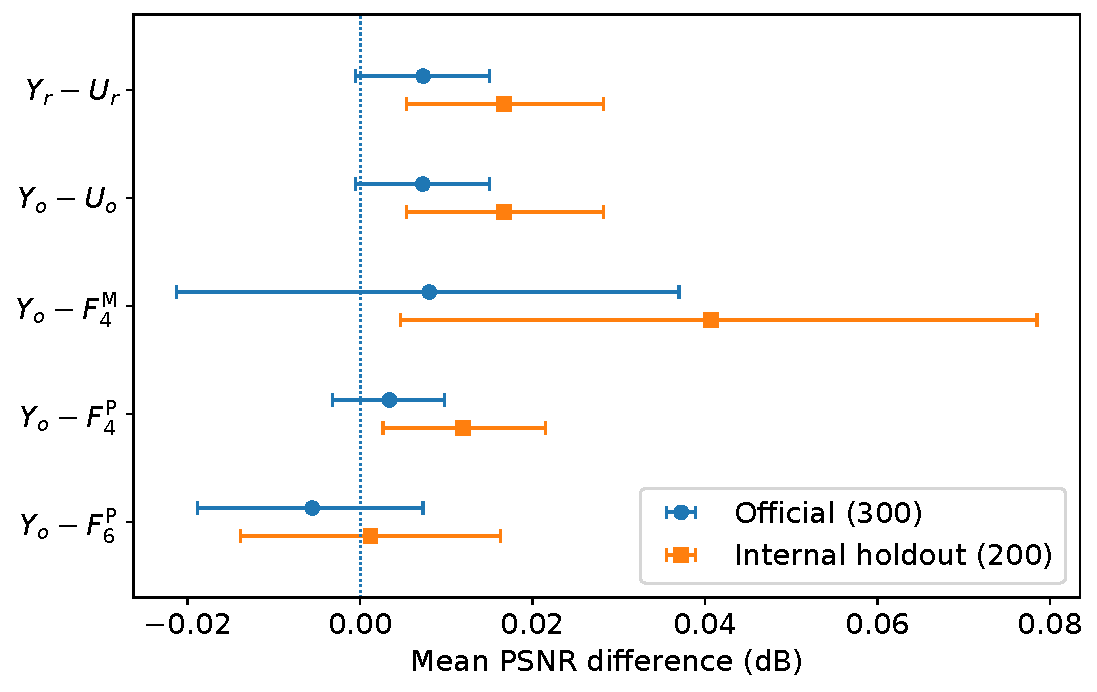
\includegraphics[width=\linewidth]{figures/Fig1.pdf}
\caption{Adaptive aggregation relative to matched uniform operators and calibrated fixed mixtures on official and internal-holdout images. The first contrast matches residual-space operators; subsequent contrasts use output-space aggregation and calibration-selected fixed weights. Error bars are 95\% paired image-bootstrap intervals with calibration weights held fixed. Six-candidate controls additionally include the base and input}
\label{fig:operators}
\end{figure}

\subsection{Replayable evidence makes stronger fixed controls testable}
All 800 error Gram matrices are symmetric and positive definite at numerical precision, with minimum eigenvalue $7.17\times10^{-8}$. Direct evaluation of three prespecified mixtures and Gram replay agree within $7.93\times10^{-16}$ MSE across all records. The upper triangles require 21 float64 numbers per image: 168 bytes of numerical payload, or approximately 131 KiB over 800 images, excluding identifiers and metadata. This compact record supports calibration and loss evaluation of global mixtures without repeating model inference.

Under mean image MSE, the four-expert optimum places all weight on $E_1$. Its simplex dual gap is numerically zero, and it equals the separately selected single-expert control. The forced expert retains the bank's joint-training history, isolating an inference choice within that learned bank. Under mean PSNR, the calibrated weights are approximately $(0.0779,0.4345,0.4876,0)$ (Table~\ref{tab:weights}). The branch with the best individual selection mean PSNR is $E_3$, illustrating that the preferred individual and the preferred mixture need not share the same allocation.
\begin{table}[t]
\caption{Selection-calibrated global output-mixture coefficients}
\label{tab:weights}
\begin{tabularx}{\linewidth}{@{}Xlrrrrrr@{}}
\toprule
Mixture & Loss & $E_0$ & $E_1$ & $E_2$ & $E_3$ & $B$ & $I$\\
\midrule
$F_4^{\rm M}$ & MSE & 0.0000 & 1.0000 & 0.0000 & 0.0000 & 0.0000 & 0.0000 \\
$F_4^{\rm P}$ & PSNR & 0.0779 & 0.4345 & 0.4876 & 0.0000 & 0.0000 & 0.0000 \\
$F_6^{\rm M}$ & MSE & 0.0000 & 0.9923 & 0.0000 & 0.0000 & 0.0000 & 0.0077 \\
$F_6^{\rm P}$ & PSNR & 0.0182 & 0.5819 & 0.3739 & 0.0000 & 0.0000 & 0.0261 \\
\bottomrule
\end{tabularx}
\tabnote{Coefficients are fitted on 300 selection images and held fixed on official and internal-holdout images. $E_k$ uses the zero-based implementation index. Superscripts M and P denote arithmetic mean image MSE and mean-PSNR calibration. Four-candidate families contain only the clipped experts; six-candidate families additionally contain base and input. Rounding can affect displayed sums.}
\end{table}

\begin{table}[t]
\caption{Raw output quality under matched operators and calibrated fixed alternatives}
\label{tab:calibrated}
\begin{tabularx}{\linewidth}{@{}Xrrrr@{}}
\toprule
Method & \multicolumn{2}{c}{Official ($n=300$)} & \multicolumn{2}{c}{Internal ($n=200$)} \\ & PSNR & MSE & PSNR & MSE\\
\midrule
Base $B$ & 34.3224 & 5.9890 & 32.6214 & 11.0316 \\
Uniform residual $U_r$ & 34.4821 & 5.8030 & 32.8135 & 10.6838 \\
Adaptive residual $Y_r$ & 34.4894 & 5.8040 & 32.8302 & 10.6581 \\
Uniform output $U_o$ & 34.4821 & 5.8030 & 32.8135 & 10.6837 \\
Adaptive output $Y_o$ & 34.4894 & 5.8040 & 32.8302 & 10.6581 \\
$F_4^{\rm M}$ & 34.4814 & 5.7506 & 32.7895 & 10.6425 \\
$F_4^{\rm P}$ & 34.4860 & 5.7997 & 32.8183 & 10.6719 \\
$F_6^{\rm M}$ & 34.4885 & 5.7499 & 32.7984 & 10.6381 \\
$F_6^{\rm P}$ & 34.4949 & 5.8000 & 32.8290 & 10.6736 \\
\bottomrule
\end{tabularx}
\tabnote{PSNR is the mean image-wise score in dB (higher is better); MSE is the arithmetic mean image MSE multiplied by $10^4$ (lower is better). Fixed mixtures are evaluated from the per-image Gram records. All methods use raw unit-range RGB and the same four-pixel crop. This table is separate from the historical JPEG system comparisons.}
\end{table}


The choice of calibration objective materially changes the comparison with spatial adaptation. Against $F_4^{\rm M}$, adaptive output aggregation $Y_o$ has an official mean-PSNR advantage of 0.00800 dB, but its arithmetic mean image MSE is higher by $5.34\times10^{-6}$, with interval $[1.13,9.59]\times10^{-6}$. This is approximately 0.93\% higher than the calibrated MSE. The reference loss used to select the fixed mixture therefore exposes a different ordering from mean PSNR.

Against the PSNR-calibrated $F_4^{\rm P}$, the official adaptive increment narrows to 0.00341 dB $[-0.00317,0.00975]$. Internal holdout retains 0.01190 dB $[0.00265,0.02148]$. The corresponding MSE differences are $+4.32\times10^{-7}$ and $-1.38\times10^{-6}$, with both intervals crossing zero. Calibrated comparison thus separates the contribution of spatially varying weights from the quality of a particular uniform reference rule, while retaining the error criterion governing each decision.

The six-candidate fits expose an additional action-space effect. For mean MSE, the optimum is $0.99225E_1+0.00775I$, with zero base weight. Since the solution lies on the $E_1$--input edge, its input coefficient agrees with the closed-form edge minimizer
\begin{equation}
\beta^*=\clip\!\left(\frac{\bar G_{11}-\bar G_{1I}}
{\bar G_{11}+\bar G_{II}-2\bar G_{1I}},0,1\right),
\end{equation}
where $\bar G$ averages the selection Gram matrices. The simplex optimality check confirms this solution over the full six-candidate MSE family. Mean-PSNR calibration assigns 2.61\% weight to the input, redistributes the expert coefficients, and again gives zero weight to the base.

Relative to the corresponding four-expert fit, $F_6^{\rm P}$ gains 0.00897 dB on official validation and 0.01069 dB on internal holdout. The observed official mean-PSNR ordering then favors $F_6^{\rm P}$ over $Y_o$ by 0.00556 dB; the paired interval includes zero. These are comparisons between different action sets, with unconditional input mixing in the fixed family. Image-dependent preservation decisions are a further question, addressed geometrically in Section~\ref{sec:control-results}.

\subsection{Aggregation redistributes losses across images}
At the 0.1 dB base-relative threshold, official losses fall from 25 under $U_r$ to 12 under $Y_r$. Fourteen images leave the loss set and one enters it. The paired rate difference is $-4.33$ percentage points, with interval $[-7.00,-2.00]$. Fig.~\ref{fig:harm} shows the threshold profile alongside calibrated alternatives.
\begin{figure}[t]
\centering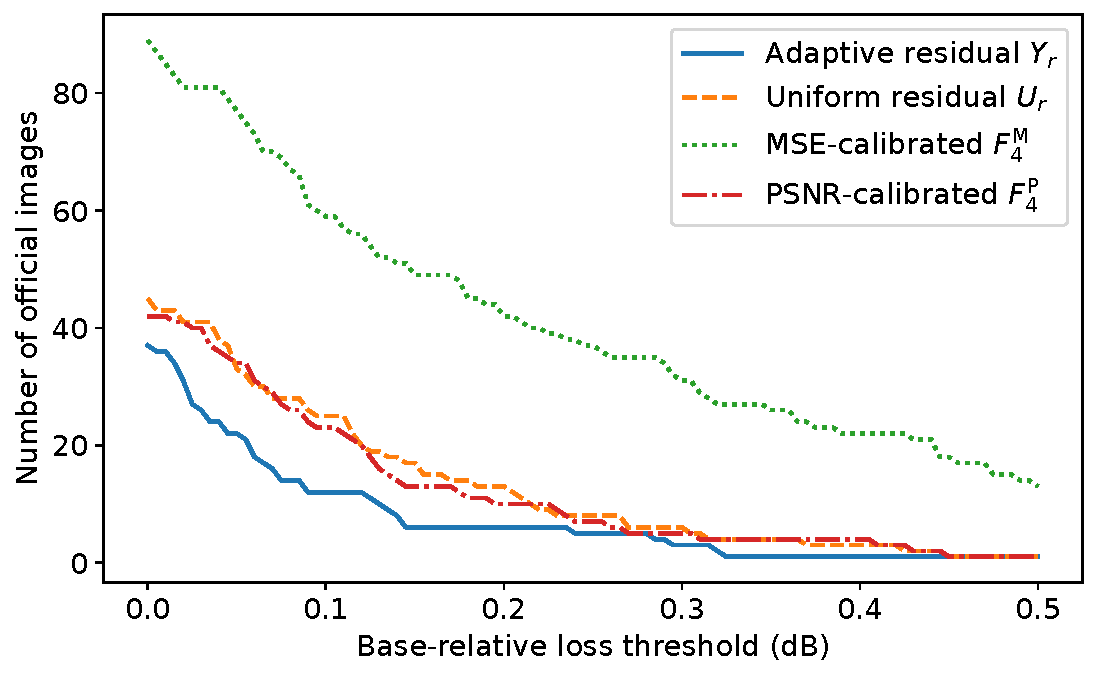
\includegraphics[width=\linewidth]{figures/Fig2.pdf}
\caption{Official raw base-relative loss profiles. Adaptive and uniform residual aggregation use matched clipping order. Fixed four-expert mixtures are calibrated on selection for MSE or mean PSNR. The horizontal axis is a numerical reporting threshold, and each curve counts the images whose gain over the base falls below its negative}
\label{fig:harm}
\end{figure}

The gain--loss decomposition localizes the mean weighting effect. Uniform residual aggregation has $G^+=0.18310$ dB and $G^-=0.02344$ dB; adaptive aggregation has $G^+=0.18039$ dB and $G^-=0.01342$ dB. The 0.00730 dB increment is therefore the net result of approximately 0.01002 dB less negative burden and 0.00271 dB less positive gain. This describes redistribution over the observed images rather than a uniform improvement of each prediction.

The same measurements preserve variation across partitions. Selection losses at 0.1 dB increase from 22 to 23, with three rescued and four introduced cases. Internal-holdout losses decrease from 17 to 13, with six rescued and two introduced cases; its paired rate interval includes zero. The strongest threshold-specific reduction occurs on official validation.

Arithmetic mean image MSE supplies a complementary summary. Official $Y_r$ has MSE $5.804016\times10^{-4}$ versus $5.802979\times10^{-4}$ for $U_r$, approximately 0.0179\% higher despite its positive mean-PSNR increment. The paired MSE interval includes zero. Table~\ref{tab:calibrated} shows this small reversal alongside the larger loss-specific differences exposed by calibrated mixtures. Together, these comparisons make the objective of aggregation explicit: mean logarithmic fidelity, absolute squared error, and thresholded loss rates describe different aspects of the same error distribution.

\subsection{Position in the wider accuracy--capacity landscape}
Table~\ref{tab:capacity} compares eleven public systems and the principal in-house systems. KLETech-CEVI reaches 34.538 dB with 27.4 million reported parameters. JOME uses approximately 9.6\% fewer parameters and is 0.1902 dB lower in historical JPEG PSNR. The retained paired interval for JOME minus KLETech-CEVI is $[-0.4234,0.0410]$ dB. RRay reaches 36.169 dB with 322.82 million reported parameters and additional paired data, a 1.8216 dB advantage over JOME. The five other leading released systems also exceed JOME overall.
\begin{table}[t]
\caption{Complete parameter context for the public technical-specification entries and the principal in-house systems}
\label{tab:capacity}
\begin{tabularx}{\linewidth}{@{}Xrcr c@{}}
\toprule
Method & Parameters M & Data & PSNR & Source\\
\midrule
refineX & 8.20 & O & 30.599 & P \\
PAST & 21.74 & O & 34.191 & I \\
JOME & 24.76 & O & 34.347 & I \\
ARISE & 24.80 & O & 34.226 & I \\
SiGMoid & 26.13 & O & 34.279 & P \\
KLETech-CEVI & 27.40 & O & 34.538 & L \\
PSU & 45.60 & O & 34.515 & P \\
NTR & 142.50 & O & 33.968 & P \\
ACVLAB & 267.17 & O & 31.689 & P \\
AIIALab & 314.00 & O+ & 35.380 & L \\
RRay & 322.82 & O+ & 36.169 & L \\
VIP Lab & 404.00 & O+ & 34.687 & L \\
YuFans & 522.34 & O & 34.906 & L \\
Xreflect Master & 545.52 & O+ & 36.050 & L \\
\bottomrule
\end{tabularx}
\tabnote{O: reported OpenRR paired training only; O+: reported additional paired data. These labels summarize reported paired-data use; broader pretraining varies by provider. I: local in-house JPEG evaluation; L: local evaluation of released outputs; P: published aggregate score without a retained output set. Public counts and P scores come from the versioned NTIRE report described in Section~\ref{sec:protocol}; parameter counts retain their reported values. Hardware, training budgets, and inference procedures are unmatched. Rows are sorted by parameter count.}
\end{table}


These measurements locate the controlled experiment within the observed performance landscape. The operator analysis adds information orthogonal to that ranking: it identifies the share of refinement gain already available in a fixed bank, measures the effect of adaptive weights under competing loss objectives, and makes the input-relative consequence of the selected output explicit. The same comparisons can be applied to stronger candidate banks when their matched outputs and cross-candidate evidence are retained.

\section{Input-relative outcomes and the geometry of available edits}
\label{sec:control-results}
\subsection{Stagewise improvement and complete-pipeline benefit}
The two-baseline view makes the consequence of a correction explicit (Table~\ref{tab:quadrants}). In the controlled raw evaluation on official validation, 257 JOME outputs improve both the base and the input, six improve only the base, 29 improve only the input, and eight improve neither. The pipeline improves 286 of 300 inputs. The historical JPEG counts are 257, five, 29, and nine, respectively, illustrating the value of preserving representation-specific evidence.
\begin{table}[t]
\caption{Two-baseline outcomes for the controlled raw JOME predictions}
\label{tab:quadrants}
\begin{tabularx}{\linewidth}{@{}Xrrrr@{}}
\toprule
Partition ($n$) & Both & Base only & Input only & Neither\\
\midrule
Selection (300) & 250 & 10 & 27 & 13 \\
Official (300) & 257 & 6 & 29 & 8 \\
Internal holdout (200) & 172 & 0 & 19 & 9 \\
\bottomrule
\end{tabularx}
\tabnote{Columns identify positive PSNR gains against the base and input. Every image has nonzero gain in both comparisons. For historical official JPEG outputs the corresponding counts are 257, 5, 29, and 9; representations are kept distinct.}
\end{table}

\begin{figure}[t]
\centering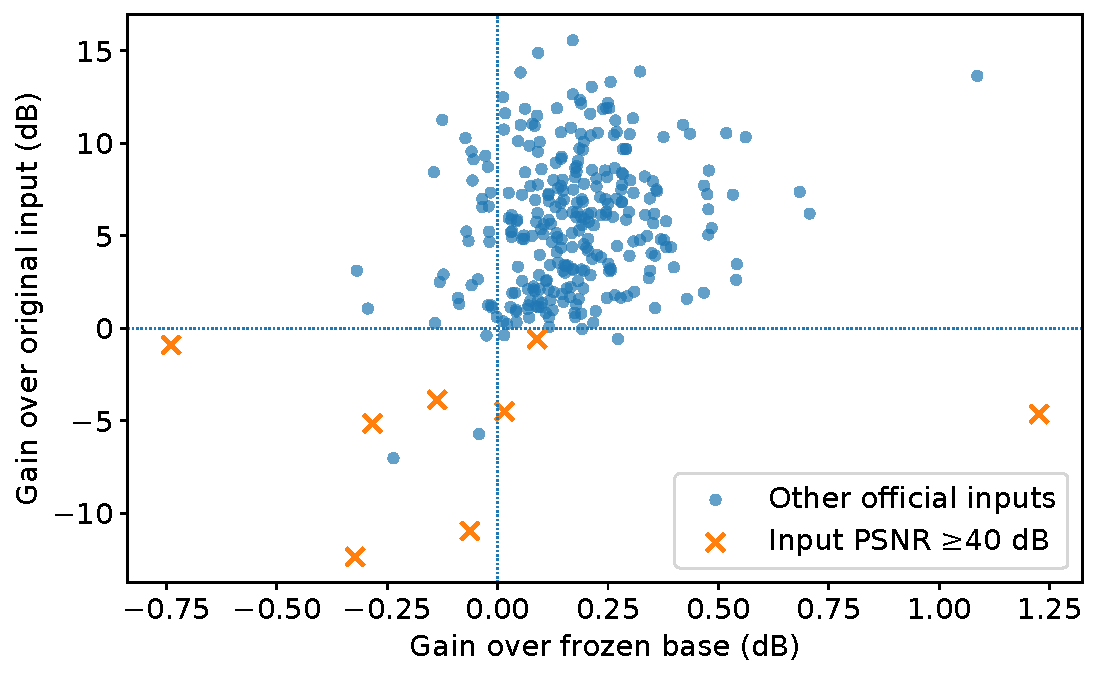
\includegraphics[width=\linewidth]{figures/Fig3.pdf}
\caption{Official raw JOME gains relative to the frozen base and the original input. Each point is an image; crosses mark the eight reference-defined near-identity inputs. The quadrants distinguish refinement-stage progress from complete-pipeline benefit. All points come from the same controlled inference pass}
\label{fig:baselines}
\end{figure}

For image \texttt{val\_0248}, the controlled raw prediction improves over the base by 1.226 dB while remaining 4.646 dB below the input. The correction repairs part of the base error, and direct preservation remains preferable under the supplied reference. Fig.~\ref{fig:baselines} places such examples in the full image-wise distribution rather than treating them as representative of every input.

A reference-aware choice among the finite actions $\{I,B,Y\}$ selects the input for 14 official images, the base for 29, and JOME for 257. Its mean-PSNR gain over the deployed prediction is 0.19785 dB, with paired interval $[0.07845,0.34792]$. The corresponding gains are 0.25039 dB on selection and 0.13755 dB on internal holdout. These values describe reference-conditioned headroom within the stated three-action set. A deployable selector would estimate the appropriate action from available input features and would be evaluated under a separate calibration protocol.

The selected photographic examples provide complementary visual context (Fig.~\ref{fig:photos}). The second and third examples show visible suppression of reflections, while the differences between base and correction are subtle elsewhere. A high global input PSNR can coexist with localized reflection structure, as in the sky of the first example. The final near-identity example, \texttt{val\_0248}, connects the two-baseline score disagreement described above to visually subtle edits. Reference-relative near-identity membership therefore describes an image-level measurement; the reference score alone does not establish perceptual preference, and regional fidelity requires its own evidence.
\begin{figure}[t]
\centering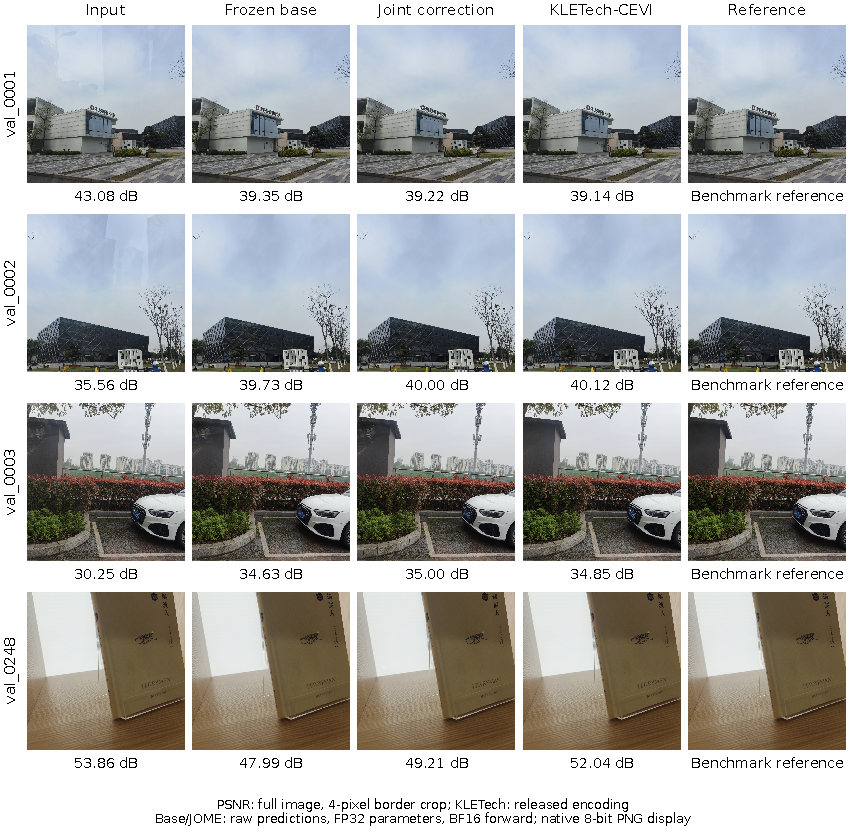
\includegraphics[width=\linewidth]{figures/Fig4.pdf}
\caption{Four purposefully selected official examples: input, frozen base, JOME, KLETech-CEVI, and reference. PAST/JOME panels are native-size 8-bit PNG display copies of the model predictions; their labels use raw floating-point predictions with a four-pixel border crop. KLETech-CEVI panels and labels use its original released encoding. Inputs and targets are from OpenRR \citep{cai2025openrr}; external outputs retain their provider attribution}
\label{fig:photos}
\end{figure}

\subsection{Input-recovery geometry is measurable}
The nominal $\epsilon=0.1$ input-recovery bound is positive for 295 of 300 selection images, 284 of 300 official images, and 194 of 200 internal-holdout images: 773 of 800 overall (Table~\ref{tab:reachability}). On official validation its mean is $4.18\times10^{-4}$ MSE, median $6.83\times10^{-5}$, and maximum $6.67\times10^{-3}$. The affected RGB coordinates occupy 2.44\% of an image on average. Reporting both activity and magnitude distinguishes exact recovery geometry from the scale of the excluded displacement.
\begin{table}[t]
\caption{Measured input-recovery geometry at nominal correction radius $\epsilon=0.1$}
\label{tab:reachability}
\begin{tabularx}{\linewidth}{@{}Xrrrr@{}}
\toprule
Partition & Active bound & Mean bound & RGB \% & Loss subset\\
\midrule
Selection & 295/300 & 5.674 & 3.60 & 23/23 \\
Official & 284/300 & 4.182 & 2.44 & 10/14 \\
Internal holdout & 194/200 & 7.626 & 3.40 & 9/9 \\
\bottomrule
\end{tabularx}
\tabnote{Active bound counts images with a strictly positive lower bound in Eq.~\eqref{eq:reachable-bound} for $X=I$. Mean bound is MSE multiplied by $10^4$; RGB \% is the image-wise mean fraction of affected RGB coordinates. Loss subset counts active bounds among outputs worse than the input. Positivity measures exact input-recovery geometry; magnitude and target-relative losses are reported separately. The floating-point envelope audit is described in the text.}
\end{table}


A large correction from the input is often useful, so bound activity is interpreted together with target-relative outcomes. Ten of the 14 official outputs worse than the input have a positive bound; five of the eight official near-identity inputs do so. The remaining adverse cases demonstrate that the coordinate envelope alone does not diagnose every loss. Availability of the original observation and quality of the selected correction remain complementary evaluation questions.

Finite precision is visible at the scale of the amplitude constraint. The executed correction exceeds the nominal coordinate radius on nine selection and six internal-holdout images, with maximum excess $9.77\times10^{-5}$; no official image has such an excess. Router weight sums differ from one by at most $2.38\times10^{-7}$. Both the nominal bound comparison and the recorded output-envelope-adjusted comparison pass on all 800 records at tolerance $10^{-10}$ MSE, and their positive-bound counts agree. The adjusted radius uses each executed output's observed maximum displacement and is consequently an output-level consistency check. The all-action statement in Proposition~\ref{prop:reachability} applies when each candidate and the weights satisfy its stated constraints. Keeping these two levels explicit makes numerical implementation part of the geometric evaluation.

An input candidate gives a direct architectural response to this geometry. It adds a reproducible unchanged-observation action even when the base-centered residual family excludes exact recovery. The calibrated six-output mixtures in Section~\ref{sec:capacity-results} exercise one global use of that action. The finite-action diagnostic above shows where a reference-aware image-level choice would differ from always executing JOME.

\subsection{Input fidelity, edit direction, and strength}
The official reference-defined input-PSNR strata contain 65, 114, 82, 31, and eight images. Controlled raw JOME mean input gains are 8.873, 6.009, 3.698, 3.399, and $-5.376$ dB across those strata. RRay exceeds JOME in every displayed stratum, including the near-identity group (Fig.~\ref{fig:conditional}). Thus the conditional analysis identifies a high-input-fidelity regime of reduced benefit while preserving the observed external performance ordering.
\begin{figure}[t]
\centering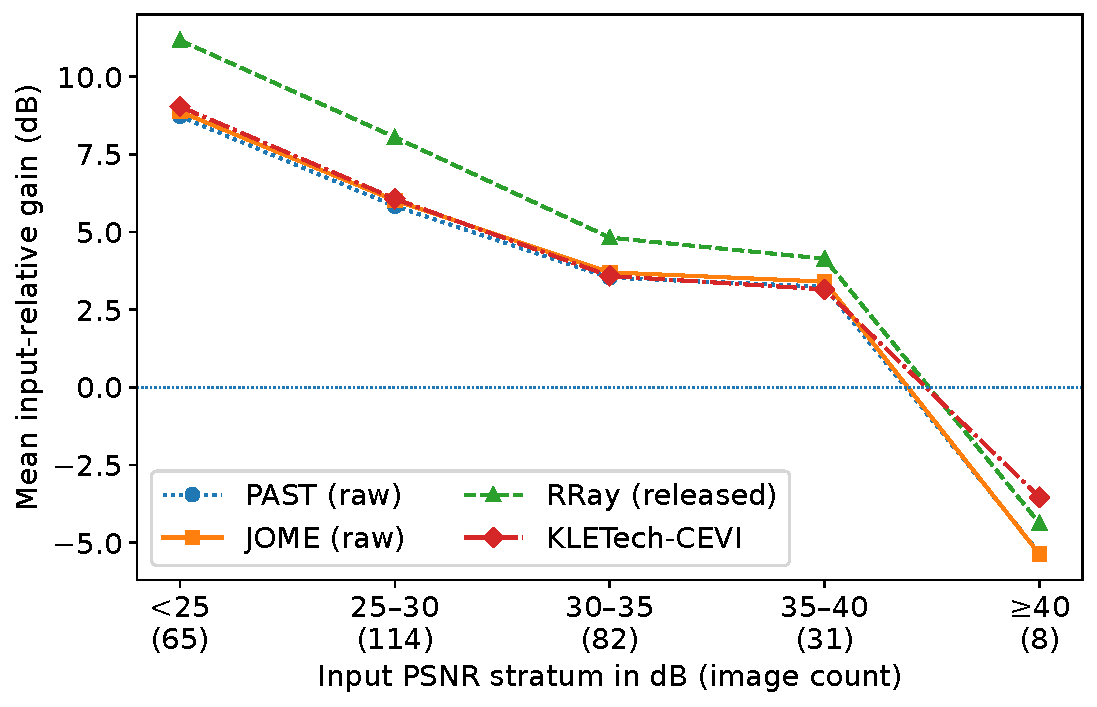
\includegraphics[width=\linewidth]{figures/Fig5.pdf}
\caption{Input-relative mean PSNR gains in disjoint reference-defined strata. PAST/JOME use the controlled raw pass; RRay and KLETech-CEVI use their released encodings. Stratum sizes are 65, 114, 82, 31, and eight. Binning is retrospective and uses the reference. The final stratum motivates direct analysis of edit magnitude and input-preserving actions}
\label{fig:conditional}
\end{figure}

Let $e=T-I$ be the reference displacement and $c=Y-I$ the applied edit. Their geometry gives
\begin{equation}
q=\MSE(Y,T)-\MSE(I,T)=\|c\|^2-2\langle c,e\rangle.\label{eq:correction-geometry}
\end{equation}
For nonzero norms, define $r=\|c\|/\|e\|$ and $\rho=\langle c,e\rangle/(\|c\|\|e\|)$. Improvement requires $r<2\rho$. Positive alignment can coexist with excess edit strength because direction and magnitude enter the error separately.

For attenuation along the recorded edit, $Y_\lambda=I+\lambda c$, $0\leq\lambda\leq1$, write $a=\|e\|^2$, $b=\|c\|^2$, and $d=\langle c,e\rangle$. Then
\begin{equation}
\MSE(Y_\lambda,T)=a+\lambda^2b-2\lambda d,\qquad
\lambda^\star=\clip(d/b,0,1),\label{eq:strength}
\end{equation}
for $b>0$. The interpolation stays inside the valid image box and is evaluated without additional clipping or serialization. The optimum uses the reference and describes the best retrospective strength along the given edit direction.

All eight official near-identity JOME edits have positive alignment and all eight lower PSNR relative to the input. Their median $\lambda^\star$ is 0.109; the corresponding base median is 0.105. Both systems have strictly interior optimal strengths for every image in this subgroup. Across the seven released systems, all 56 analogous edits also align positively, 54 lower PSNR, and every optimal strength lies strictly between zero and one (Table~\ref{tab:geometry}). Positive direction coupled with excessive magnitude is therefore a shared property of these stored near-identity edits.
\begin{table}[t]
\caption{Correction strength and reference-space margins on eight official near-identity inputs}
\label{tab:geometry}
\begin{tabularx}{\linewidth}{@{}Xrrrr@{}}
\toprule
Method & Gain dB & Losses & Median $\lambda^\star$ & Median $255\eta^\star$\\
\midrule
PAST (raw) & -5.349 & 8/8 & 0.105 & 0.786 \\
JOME (raw) & -5.376 & 8/8 & 0.109 & 0.791 \\
RRay & -4.379 & 8/8 & 0.164 & 0.669 \\
Xreflect Master & -5.163 & 8/8 & 0.137 & 0.734 \\
AIIALab & -4.854 & 7/8 & 0.128 & 0.776 \\
VIP Lab & -6.853 & 8/8 & 0.105 & 0.905 \\
YuFans & -6.026 & 8/8 & 0.109 & 0.915 \\
KLETech-CEVI & -3.540 & 7/8 & 0.160 & 0.679 \\
OPPO baseline & -8.499 & 8/8 & 0.098 & 1.360 \\
\bottomrule
\end{tabularx}
\tabnote{JOME and PAST use the controlled raw predictions; other systems retain their released encodings. All 72 image--system edits have positive target alignment. $\lambda^\star$ is the reference-conditioned optimal attenuation; $\eta^\star$ is the unconstrained RMS distance to an equal-loss reference. These reference-based diagnostics characterize the stored images and action directions.}
\end{table}


One global attenuation produces a tradeoff across populations. For JOME, $\lambda=0.1$ changes the official near-identity mean gain from $-5.376$ to $+0.203$ dB, while reducing the complete-set gain from 5.425 to 0.573 dB. RRay at $\lambda=0.25$ changes the subgroup from $-4.379$ to $+0.440$ dB and the complete set from 7.105 to 1.790 dB. The curves in Fig.~\ref{fig:strength} show how a common control couples improvements on a small high-fidelity population to reduced benefit elsewhere.
\begin{figure}[t]
\centering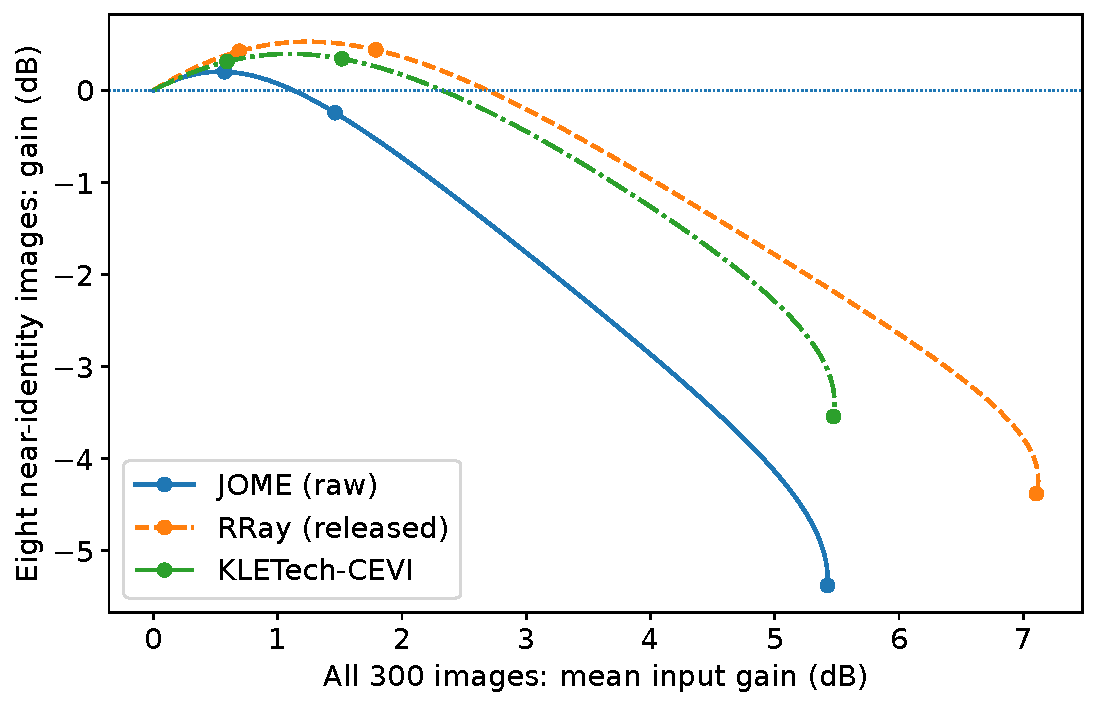
\includegraphics[width=\linewidth]{figures/Fig6.pdf}
\caption{Retrospective global-strength tradeoffs for JOME, RRay, and KLETech-CEVI. Each curve applies the same $\lambda$ to all 300 outputs and compares complete-set with eight-image near-identity gains. Markers indicate $\lambda=0.1$, $0.25$, and $1$. Curves are reconstructed from per-image geometry; they evaluate output interpolation rather than a learned input-dependent strength policy}
\label{fig:strength}
\end{figure}

The smaller subgroups in the other partitions have different compositions. Internal holdout contains five near-identity inputs, with JOME mean gain $+0.674$ dB and median optimal strength 0.632. Selection contains four, with mean gain $-2.825$ dB and median strength 0.450. These variations make subgroup size, individual records, and threshold sensitivity important alongside aggregate curves. Controllable restoration designs such as CURE \citep{kim2026cure} provide a natural connection: exposing a strength coordinate creates an action space, and evaluating how an action is selected establishes its utility for each input population.

\subsection{Reference-space margins contextualize numerical preference}
Edited targets motivate a complementary sensitivity question: how far must the reference move before the relative preference between output and input changes? Replacing $T$ by $T+\delta$ in Eq.~\eqref{eq:correction-geometry} gives
\begin{equation}
q'=q-2\langle c,\delta\rangle,\qquad |q'-q|\leq2\|c\|\,\|\delta\|.\label{eq:reference-sensitivity}
\end{equation}
For $c\ne0$, the unconstrained RMS distance to the equal-loss reference hyperplane is
\begin{equation}
\eta^\star=\frac{|q|}{2\|c\|}.\label{eq:reference-radius}
\end{equation}
Equality is attained by $\delta=q\,c/(2\|c\|^2)$, and any smaller RMS perturbation preserves the sign of a nonzero $q$. Requiring the alternative reference to remain in the image box can increase this distance. Each minimizing perturbation depends on the image and model.

For official near-identity JOME outputs, the median $255\eta^\star$ is 0.791 in 8-bit channel units; the base median is 0.786. The six leading released systems range from 0.669 to 0.915, and the OPPO baseline is 1.360. These radii place a reference-relative dB loss alongside the geometric margin of the preference it expresses. They are distances in reference space; connecting them to actual target variation calls for repeated or independently acquired references. Regional annotations and perceptual evaluation would further connect the numerical preference to physical content preservation and viewer utility.

\section{Implications for restoration research}
\label{sec:discussion}
\subsection{Adaptive aggregation needs an operator and a loss objective}
The controlled results organize refinement gain into an interpretable sequence. Joint training produces a useful bank of corrections. Uniform residual aggregation makes most of the mean gain available. Adaptive weighting changes the distribution of those gains and losses, and calibrated alternatives show how much of that change depends on the comparator and its loss objective. This sequence addresses practical decisions about which predictions to retain and which aggregation to deploy.

The four-operator experiment gives the comparison a concrete meaning. Clipping order is measured directly, and its interaction with weighting is small for these recorded predictions. The official 0.0073 dB matched weighting increment can therefore be interpreted alongside its distributional consequence: approximately 0.0100 dB less negative burden and 0.0027 dB less positive gain. Its mean-MSE ordering and cross-partition loss profiles differ, so a single positive mean increment does not specify the entire objective achieved by aggregation.

Calibration strengthens the measurement. MSE selects one expert, whereas mean PSNR selects a multi-expert combination. Against the latter, the official adaptive increment contracts to 0.0034 dB. The comparator thus embodies a decision criterion rather than serving as a neutral default. Evaluation of a modular predictor becomes more informative when candidate membership, clipping order, loss aggregation, calibration population, and deployment-available information are reported together.

\subsection{Compact loss evidence enables substantive reuse}
Per-image error Gram matrices allow global output-mixture losses to be recomputed without repeating network inference. The 21 retained cross-products per image support both convex MSE calibration and numerical PSNR calibration, with all coefficients frozen outside selection. Their direct replay check ties the abstraction to actual output mixtures. This is a concrete consequence of the scalar-score insufficiency result: retaining cross-candidate information permits comparisons that individual scores and a uniform average leave undetermined.

The value of this record is operator-specific. Global linear output mixtures are exactly represented; spatial routing and residual mixing followed by clipping call for different retained evidence. An evaluation can therefore specify its intended family of alternative decisions before choosing what to store. Checkpoints enable a rerun, while sufficient statistics make a declared family of loss comparisons inexpensive to revisit. Their roles complement each other.

\subsection{Preserving an observation is an action-space decision}
The input-recovery analysis connects content preservation to architecture. A bounded refiner operates around the base prediction, while the original input can lie outside its nominal correction region. Measuring the bound together with input-relative losses distinguishes availability of the observation from the quality of the chosen edit. The official six base-only improvements exemplify why the original input and unchanged base deserve separate treatment.

The six-candidate calibration makes one use of the added input action, through a small global coefficient. The finite-action reference diagnostic quantifies a different possibility, selecting among input, base, and JOME for each image. Strength geometry then adds a continuum of retrospective actions. These comparisons organize control into three questions: which outputs the architecture permits, how the selection rule uses available information, and how the resulting edit is evaluated. Each question has a corresponding evidence requirement.

Reference margins provide further context for high-fidelity inputs. JOME and the released systems can align their edits positively with the target displacement while applying excessive magnitude. The optimal strength and equal-loss margin describe this geometry without assigning a physical cause to the benchmark reference. Together, they connect numerical preference to the acquisition and target-construction process that a broader preservation evaluation would measure.

\subsection{Evaluation conditions and the next empirical tests}
The empirical findings concern selected checkpoints and retrospective OpenRR partitions. The paired intervals quantify image-wise variation conditional on those checkpoints and calibrated coefficients; scene identifiers and calibration resampling would be needed to characterize additional sources of uncertainty. The small near-identity subgroups differ substantially across partitions. An independently sourced, overlap-audited, scene-separated evaluation is therefore the most direct test of the stability of the observed loss profiles.

The controlled raw pass supplies matched weighting--clipping evidence, calibrated output mixtures, and measured base/JOME geometry. A globally calibrated residual-then-clip family would extend the fixed controls into the deployment operator itself and requires pre-clipping tensors or renewed inference. A selector over input, base, and restoration strengths would connect the available actions to decisions based on observable features. Repeated reference construction, regional fidelity measurements, and identity-control inputs would then test the correspondence between reference-based improvement and preservation. Component profiling and resource-matched training comparisons would address the separate role of candidate generation and execution cost.

The analytical framework applies to image-valued corrections satisfying its operator assumptions. Its empirical realization here is reflection removal; task-specific references and matched controls are required when carrying the evaluation to other restoration problems. In this form, the framework supplies a reusable experimental design for studying how modular prediction systems turn a bank of possible corrections into an intervention on an observation.

\section{Conclusion}
This paper develops and exercises an operator-aware framework for evaluating correction capacity, aggregation behavior, and input-relative control. Four matched inference operators isolate adaptive weighting from clipping order. Cross-candidate error records make loss-specific global mixtures replayable, and calibrated comparisons expose the dependence of aggregation results on their objective. Input-recovery bounds and correction geometry connect the selected prediction to both the architecture's action region and the observation it changes.

The residual-expert experiment shows how useful candidates, a modest adaptive increment, and heterogeneous input-relative outcomes coexist. Reporting these properties together transforms a final accuracy score into an account of where improvement arises, which alternatives remain competitive, and which actions support preservation. Explicit operators, declared losses, and sufficient retained evidence provide the basis for that account and for its reuse in subsequent restoration research.

\section*{Declarations}
\noindent\textbf{Funding.} This work was supported by the China Vocational Education Society (Grant No.\ ZJS2026YB59) and the Basic Scientific Research Project of Liaoning Province (Grant No.\ LJ242514473001).

\noindent\textbf{Competing interests.} The author declares no competing interests.

\noindent\textbf{Author contributions.} Ruizi Wang is the sole author and has reviewed and approved the manuscript and all accompanying materials.

\noindent\textbf{Ethics and permissions.} This study used the existing public OpenRR benchmark and involved no new data collection. The benchmark and external released outputs are attributed to their original providers.

\noindent\textbf{Data and code availability.} The reproducibility package provides PAST, JOME, and ARISE evaluation checkpoints; per-image scores and error Gram matrices; base/JOME and released-output geometry; calibration coefficients; matched-operator diagnostics; configuration and source evidence; analysis and figure-generation code; checksums; and numerical tests. These materials reproduce the tabular analyses, fixed-output calibration, and geometric calculations. The controlled inference environment and checkpoint hashes are recorded in the metadata. Benchmark image pairs and external released predictions are obtained from their original providers. Code, evaluation weights, and reproducibility data will be made available at \url{https://github.com/RuiziWang0923/operator-aware-restoration}.

\noindent\textbf{Use of AI-assisted tools.} The author used ChatGPT 5.6 Sol and ChatGPT 6 Astra for coding assistance, ChatGPT-6 Sol for \LaTeX{} typesetting, and ChatGPT-6 Pro for proofreading and phrasing. The author reviewed and approved all materials and takes responsibility for the final content.

\FloatBarrier
\bibliographystyle{unsrtnat}
\bibliography{references}
\end{document}
